\documentclass[aspectratio=169,sn-mathphys-num]{beamer}

\usepackage{fontspec}
\usepackage{unicode-math}
\usepackage{graphicx}
\usepackage[dvipsnames]{xcolor}
\usepackage[sorting=none]{biblatex}
\usepackage{ragged2e}
\usepackage{setspace}
\usepackage{bookmark}
\usepackage{siunitx}
\usepackage{mhchem}
\usepackage[spanish]{babel}

\addbibresource{../references.bib}

\usetheme[numbering=counter, progressbar=frametitle, background=light]{metropolis}

\usecolortheme{dove}
\definecolor{primary}{RGB}{88, 24, 124}
\definecolor{secondary}{RGB}{0, 168, 150}

\setbeamercovered{transparent}
\setbeamercolor{frametitle}{fg=white, bg=primary}
\setbeamercolor{progress bar}{fg=secondary}
\setbeamerfont{frametitle}{size=\large, series=\bfseries}
\setbeamerfont{title}{size=\LARGE, series=\bfseries}
\setbeamercolor{alerted text}{fg=secondary}
\setbeamercolor{block title}{fg=primary}
\setbeamercolor{block body}{bg=white}

\setstretch{1.1}

\setmainfont{Fira Sans}
\setmathfont{TeX Gyre Pagella Math}

\title{Interacción Radiación-Materia}
\subtitle{Selección de Materiales de Blindaje}
\author{Herrera, Avila, Acuña, Martinez}
\institute{Universidad Distrital Francisco José de Caldas}
\date{\today}

\begin{document}

\begin{frame}
	\titlepage
\end{frame}

\begin{frame}{Definición de Radiación}
  \textbf{Radiación:} Emisión y propagación de energía a través del
  espacio o de un medio material en forma de \alert{Ondas electromagnéticas} o
  \alert{Partículas subatómicas}.
  \vfill
  \begin{columns}[T]
    \begin{column}{0.48\textwidth}
      \begin{block}{Radiación Electromagnética}
        Energía en forma de ondas. Fotones.
        \begin{itemize}
          \item Luz visible
          \item Ondas de radio
          \item Rayos X
          \item Rayos gamma ($\gamma$)
        \end{itemize}
      \end{block}
    \end{column}

    \begin{column}{0.48\textwidth}
      \begin{block}{Radiación de Partículas}
        Partículas con masa y alta velocidad.
        \begin{itemize}
          \item Partículas alfa ($\alpha$)
          \item Partículas beta ($\beta$)
          \item Neutrones
          \item Protones
        \end{itemize}
      \end{block}
    \end{column}
  \end{columns}
  \vfill

  La radiación de alta energía es \alert{ionizante}: Suficiente energía
  para desligar electrones de los átomos, alterando la materia.
\end{frame}

\begin{frame}{Interacciones Electromagnéticas con la Materia}
  Diferentes regiones del espectro electromagnético, diferentes sus efectos e
  interacciones con la materia.

  Si \alert{fotones} penetran un medio material, existen dos mecanismos de
  atenuación:
  \begin{itemize}
    \item \textbf{Difusión:} El fotón es desviado, sin
      depositar energía en el medio.
    \item \textbf{Absorción:} El fotón transfiere energía a las partículas
      cargadas, causando ionización.
  \end{itemize}
\end{frame}

\begin{frame}{Ilustración interacción radiación-materia}
  \begin{figure}
    \centering
    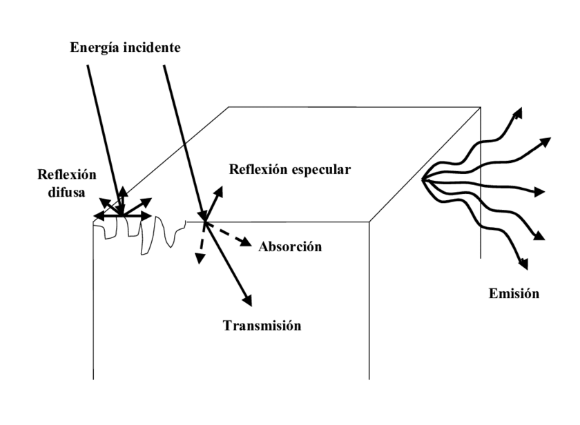
\includegraphics[width=0.6\linewidth]{../images/types_radiation.png}
    \caption{Representación de diferentes procesos ocurridos en la interacción radiación-materia.}
    \label{fig:types_radiation}
  \end{figure}
\end{frame}

\begin{frame}{Interacciones Electromagnéticas}
  El dominio de cada mecanismo depende de la energía del fotón ($E$) y del
  número atómico ($Z$) del material:

  \begin{itemize}
    \item \textbf{Efecto Fotoeléctrico:} Domina bajas energías.
    \item \textbf{Efecto Compton:} Domina a energías intermedias.
    \item \textbf{Producción de Pares:} Domina a energías altas ($>\qty{1.022}{
      \mega\eV}$).
  \end{itemize}
\end{frame}

\begin{frame}{Dominios de Interacción}
  \begin{figure}
    \centering
    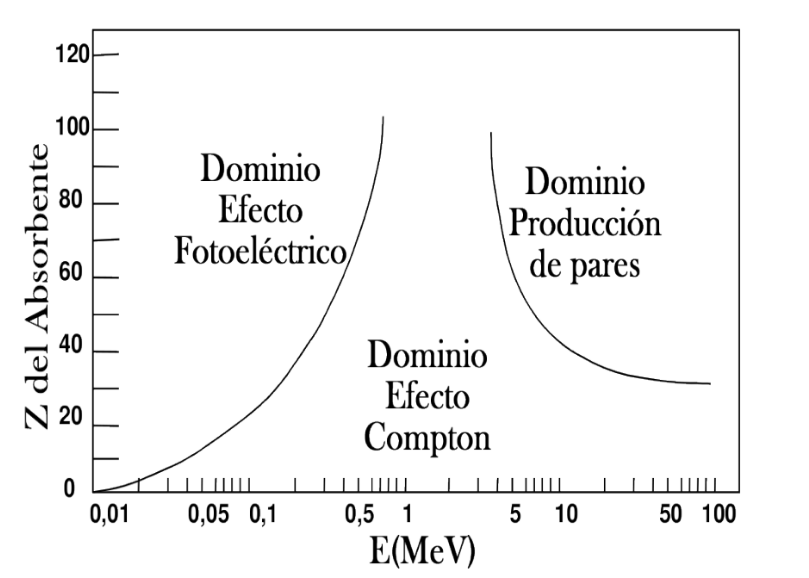
\includegraphics[width=0.6\linewidth]{../images/domains.png}
    \caption{Esquema de las regiones de dominio de los mecanismos de absorción
    de energía.}
    \label{fig:domains}
  \end{figure}
\end{frame}

\begin{frame}{Atenuación de fotones}
  La atenuación en un material homogéneo se describe por:
  \begin{block}{Ley de Beer-Lambert}
    $$I(x) = I_0 e^{-\mu x}$$
  \end{block}
  \begin{itemize}
    \item $I$ la intensidad tras pasar un grosor $x$.
    \item $I_0$ intensidad inicial.
    \item $\mu$ coeficiente de atenuación lineal.
  \end{itemize}

  El \alert{espesor medio} $x_{1/2} = \mu^{-1} \ln{2}$ y el \alert{coeficiente
  de atenuación} ${\rho}^{-1} \mu$ ($\rho$ densidad) son dependientes del
  material y la energía del fotón.
\end{frame}

\begin{frame}{Interacción con Partículas Cargadas}
  El paso de partículas cargadas a través de la materia se caracteriza por la
  pérdida de energía y la desviación de su trayectoria.

  \vfill
  \begin{block}{Tipos de Colisiones}
    \begin{itemize}
      \item \textbf{Con electrones atómicos:}
        \begin{itemize}
          \item \textit{Elástica}.
          \item \textit{Inelástica:} Ionización o excitación, con pérdida
            significativa de energía.
        \end{itemize}
      \item \textbf{Con núcleos atómicos:}
        \begin{itemize}
          \item \textit{Elástica}.
          \item \textit{Inelástica:} Frenado de la partícula y emisión de
            radiación (\textit{Bremsstrahlung}).
        \end{itemize}
    \end{itemize}
  \end{block}
\end{frame}

\begin{frame}{Esquema de las interacciones de partículas cargadas}
  \begin{figure}
    \centering
    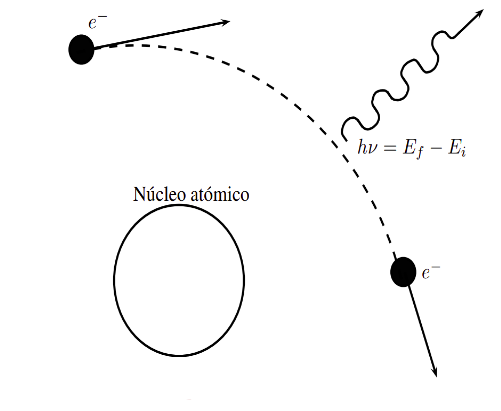
\includegraphics[width=0.55\linewidth]{../images/charged_particles.png}
    \caption{Proceso de Bremsstrahlung de un electrón de alta energía
    desviado por interacción de Coulomb del núcleo atómico.}
    \label{fig:charged_particles}
  \end{figure}
\end{frame}

\begin{frame}{Pérdida de Energía de Partículas Cargadas}
  \begin{itemize}
    \item \textbf{Por Ionización y Excitación (Fórmula de Bethe-Bloch):}
      \begin{equation*}
        -\frac{dE}{dx} = 4\pi
        r_{0}^{2}z^{2}\frac{m_{0}c^{2}}{\beta^{2}}N_{A}Z\left[\ln{\left(\frac{2m_{0}c^{2}}{I}\beta^{2}\gamma^{2}\right)}
        - \beta^{2}\right]
      \end{equation*}

    \item \textbf{Por Bremsstrahlung (Radiación de Frenado):}
      \begin{equation*}
        -\frac{dE}{dx} \approx 4\alpha N_{A}\frac{Z^{2}}{A}r_{0}^{2}E \ln{\frac{183}{Z^{1/3}}}
      \end{equation*}

    \item \textbf{Por Radiación Cherenkov:}
      \begin{itemize}
        \item Ocurre cuando una partícula viaja más rápido que la luz en ese medio.
        \item Es un mecanismo de pérdida de energía menos significativo.
      \end{itemize}
  \end{itemize}
\end{frame}

\begin{frame}{Pérdida de energía por partícula}
  \begin{figure}
    \centering
    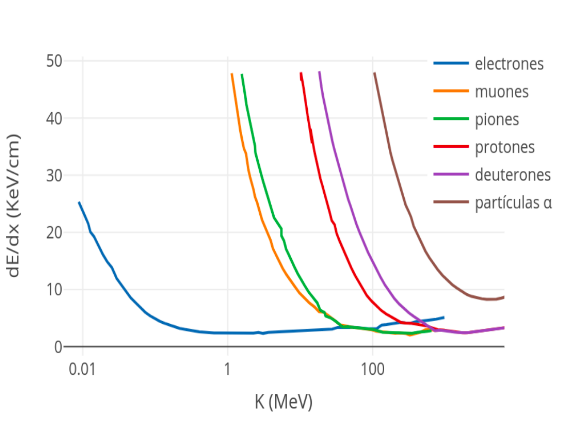
\includegraphics[width=0.6\linewidth]{../images/energy_loss.png}
    \caption{Pérdida de energía por unidad de recorrido en el plomo para
    diferentes partículas.}
    \label{fig:energy_loss}
  \end{figure}
\end{frame}

\begin{frame}{Interacciones de Neutrones}
  Los neutrones no tienen carga eléctrica, por lo que son una radiación
  \textbf{indirectamente ionizante}.

  \vfill
  \begin{block}{Proceso de Interacción}
    Interactúan mediante colisiones directas con los núcleos atómicos, generando
    partículas cargadas secundarias o fotones que sí ionizan el material.
  \end{block}

  \vfill
  Los mecanismos de interacción principales son:
  \begin{itemize}
    \item Dispersión elástica.
    \item Dispersión inelástica.
    \item Captura radiactiva.
    \item Fisión.
  \end{itemize}
\end{frame}


\input{./sections/reactor.tex}

\begin{frame}{¿Por Qué Minimizar la Masa en Aplicaciones Aeroespaciales?}
  \begin{block}{El Desafío del Reactor Espacial}
    \begin{itemize}
      \item El objetivo principal es encontrar un material que ofrezca la
        protección necesaria contra la radiación con la \textbf{mínima masa
        posible}.
      \item Esto es un problema de optimización donde se busca la mayor
        eficiencia de blindaje por unidad de masa.
    \end{itemize}
  \end{block}
  \begin{block}{Índice de Material a Optimizar}
    Para este problema, maximizamos el índice de masa mínima:
    $$ \mathcal{M}_{2} = \frac{\lambda_{eff}}{M} $$
    Donde $\lambda_{eff}$ es la atenuación y $M$ es la masa molar.
  \end{block}
\end{frame}

\begin{frame}
  \begin{figure}
    \centering
    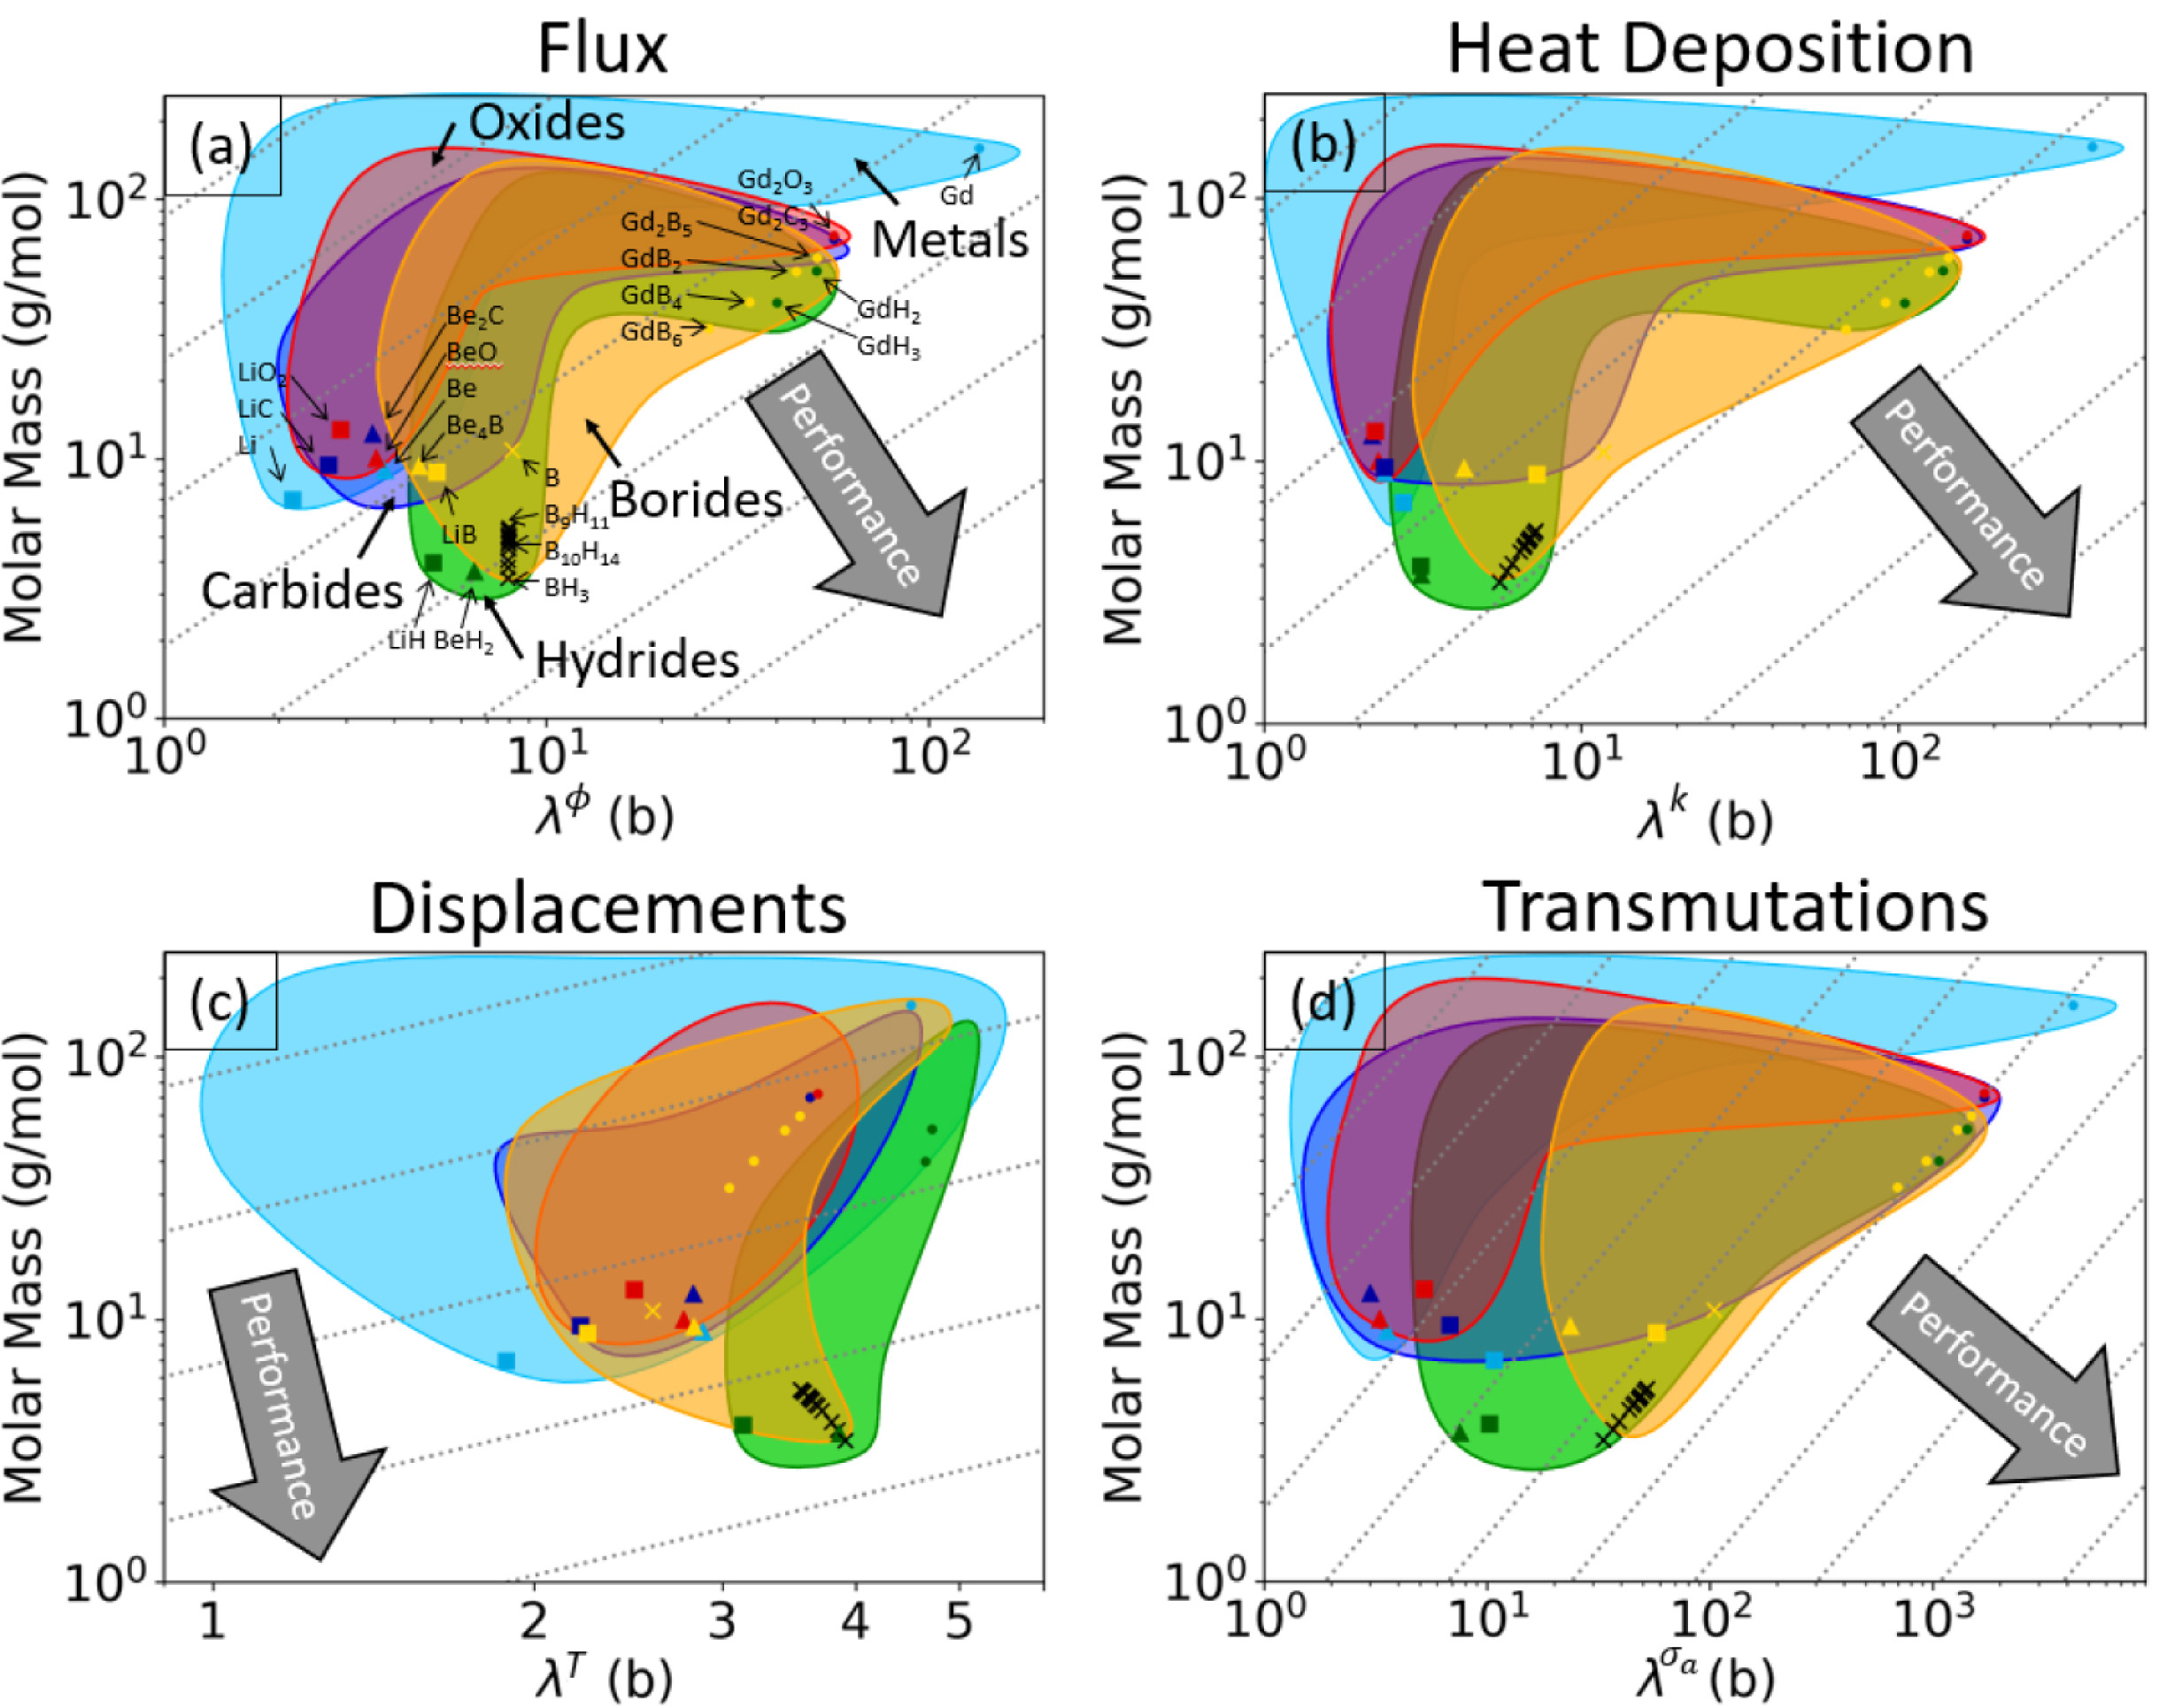
\includegraphics[width=0.65\linewidth]{../images/graph-4.jpg} 
    \caption{Materiales para blindaje de masa mínima, protegiendo
    \ce{Si} de un espectro de fisión rápido. \cite{Brand2025Material}}
  \end{figure}
\end{frame}

\begin{frame}
  \frametitle{El Material Óptimo para Proteger el Chip}
  \begin{block}{Recordando el Objetivo}
    Buscamos el material con el mayor \textbf{Índice de Material} para minimizar la masa:
    $$ \mathcal{M}_{2} = \frac{\lambda_{eff}}{M} \rightarrow \text{Maximizar}$$
  \end{block}

  \begin{alertblock}{Los Candidatos Ganadores}
    Los \textbf{Boranos} (compuestos de Boro e Hidrógeno, como \ce{B10H14}) y
    los \textbf{Hidruros} (como LiH) son los mejores materiales, superando a
    opciones más convencionales.
  \end{alertblock}
\end{frame}

\begin{frame}
  \begin{block}{¿Por Qué Son los Mejores? La Razón detrás de $\mathcal{M}_{2}$}
    \begin{itemize}
      \item \textbf{Hidruros (\ce{LiH})}: Son extremadamente ligeros (minimizan
        '$M$') y el hidrógeno es un excelente moderador de neutrones.
      \item \textbf{Boranos (\ce{B_xH_y})}: Ofrecen la mejor combinación. Tienen
        una masa molar muy baja ($M$) y un coeficiente de atenuación
        ($\lambda_{eff}$) excepcionalmente alto. Esto se debe al
        efecto combinado de la \textbf{alta absorción} de neutrones del Boro y
        la \textbf{alta dispersión} del Hidrógeno.
    \end{itemize}
  \end{block}
\end{frame}


\section{Referencias}
\begin{frame}[allowframebreaks]{References}
	\printbibliography
	\nocite{*}
\end{frame}

\begin{frame}[plain]
	\centering
	\vspace{1cm}
	{\Huge \textbf{Gracias!}}\\[1cm]
	{\large Preguntas o comentarios?}
\end{frame}

\end{document}
